\documentclass[a4paper,oneside]{bth}

\usepackage{subfiles}
\usepackage{thesis_layout}
\usepackage{amsmath}
\usepackage{mathenv}
\usepackage{amssymb}
\usepackage{amsthm}
\usepackage{textcomp}
\usepackage{longtable}
\usepackage{multirow}
\usepackage{pifont}
\usepackage{changepage}
\usepackage{listings}
\usepackage{url}
\usepackage{xspace}
\usepackage{color}
\usepackage{algorithm}
\usepackage[noend]{algpseudocode}
\usepackage{hyperref}
\usepackage{mathtools}
\usepackage{fixltx2e}
\usepackage{csquotes}
\usepackage[square]{natbib}
\usepackage{enumitem}

\usepackage{pdfpages}
\usepackage[toc,page]{appendix}

\usepackage{xtab}
\usepackage[utf8]{inputenc}
\usepackage[T1]{fontenc}
\usepackage{graphicx}
\usepackage{algorithm}
\DeclareGraphicsExtensions{.pdf}

\graphicspath{ {image/} }

\newtheorem{lem}{\textsc{Lemma}}[chapter]
\newtheorem{thm}{\textsc{Theorem}}[chapter]
\newtheorem{prop}{\textsc{Proposition}}[chapter]
\newtheorem{post}{Postulate}[chapter]
\newtheorem{corr}{\textsc{Corollary}}[chapter]
\newtheorem{defs}{\textsc{Definition}}[chapter]
\newtheorem{cons}{\textsc{Constraint}}[chapter]
\newtheorem{ex}{\textbf{Example}}[chapter]
\newtheorem{qu}{\textbf{Question}}[chapter]

\begin{document}
\tracingall
\pagestyle{plain}
\pagenumbering{roman}

% Front matter

{\pagestyle{empty}
\changepage{5cm}{1cm}{-0.5cm}{-0.5cm}{}{-2cm}{}{}{}
\noindent%   
{\small
\begin{tabular}{p{0.75\textwidth} p{0.25\textwidth}}
\textit{Master Thesis}&\multirow{4}{*}{\bthcsnotextlogo{3cm}}\\
\textit{Computer Science}\\
\textit{Thesis no: MCS-2015-NN}\\
\textit{June 2015}\\
\end{tabular}}

\begin{center}

\par\vspace {7cm}

{\Huge\textbf{Combining Regional Time Stepping With Two-Scale PCISPH Method}}  

\par\vspace {0.5cm}

%{\Large\textbf{Centered Subtitle Times Font Size 16 Bold}}                   

\par\vspace {3cm}

{\Large\textbf{Joel Begnert}}
\\
%\par\vspace {0cm}                   % Vertical space might need to be increased
{\Large\textbf{Rasmus Tilljander}}
\par\vspace {7cm}

\end{center}

\noindent%
{\small Faculty of Computing \\
Blekinge Institute of Technology\\
SE--371 79 Karlskrona, Sweden}

\clearpage
}

{\pagestyle{empty}
\changepage{5cm}{1cm}{-0.5cm}{-0.5cm}{}{-2cm}{}{}{}
\noindent%
\begin{tabular}{p{\textwidth}}
{\small This thesis is submitted to the Department of Computer Science \& Engineering at Blekinge
Institute of Technology in partial fulfillment of the requirements for the degree of Master
of Science in Computer Science. The thesis is equivalent to 20 weeks of
full-time studies.}
\end{tabular}

\par\vspace {12cm}

\noindent%
\begin{tabular}{p{0.5\textwidth}lcl}
\textbf{Contact Information:}\\
Authors:\\
Joel Begnert               & Rasmus Tilljander\\
joby10@student.bth.se      & rati10@student.bth.se\\
\par\vspace {5cm}
University advisor:\\
Dr.\ Prashant Goswami\\
Dept. Computer Science \& Engineering
\par\vspace {1cm}
\noindent%
 \\
Faculty of Computing & Internet & : & www.bth.se\\
Blekinge Institute of Technology & Phone	& : & +46 455 38 50 00 \\
SE--371 79 Karlskrona, Sweden & Fax & : & +46 455 38 50 57 \\
\end{tabular}
\clearpage
} % Back to \pagestyle{plain}

\setcounter{page}{1}


\abstract
\begin{changemargin}{+1cm}{+1cm}
\noindent
\textbf{Context}. In computer graphics, realistic looking fluid is often desired. Simulating realistic fluids is a time consuming and computationally expensive task, therefore, much research has been devoted to reducing the simulation time while maintaining the realism. Two of the more recent optimization algorithms within particle based simulations are two-scale simulation and regional time stepping (RTS). Both of them are based on the predictive-corrective incompressible smoothed particle hydrodynamics (PCISPH) algorithm. \newline
\textbf{Objectives}. These algorithms improve on two separate aspects of PCISPH, two-scale simulation reduces the number of particles and RTS focuses computational power on regions of the fluid where it is most needed. In this paper we have developed and investigated the performance of an algorithm combining them, utilizing both optimizations. \newline
\textbf{Methods}. We implemented both of the base algorithms, as well as PCISPH, before combining them. Therefore we had equal conditions for all algorithms when we performed our experiments, which consisted of measuring the time it took to run each algorithm in three different scene configurations.  \newline
\textbf{Results}. Results showed that our combined algorithm on average was faster than the other three algorithms. However, our implementation of two-scale simulation gave results inconsistent with the original paper, showing a slower time than even PCISPH. This invalidates the results for our combined algorithm since it utilizes the same implementation. \newline
\textbf{Conclusions}. We see that our combined algorithm has potential to speed up fluid simulations, but since the two-scale implementation was incorrect, our results are inconclusive. 


\par\vspace {1cm}
% 3-4 keywords, maximum 2 of these from the title, starts 1 line below the
% abstract.
\noindent
\textbf{Keywords:} smooth particle hydrodynamics, two-scale, regional time stepping, fluid simulation 

\end{changemargin}

%\include{acknowledgments} %OPTIONAL
\listoffigures %in case you have them
\listoftables %in case you have them
\listofalgorithms %in case you have them
\tableofcontents 

\cleardoublepage
\pagestyle{headings}
\pagenumbering{arabic}

\chapter{Introduction}
\subfile{\sectionIntroFile}

\chapter{Background and Related Work}
\subfile{\sectionRelatedWorkFile}

\chapter{Method}
\subfile{\sectionAimAndObjectivesFile}

\chapter{Base Algorithms}
\subfile{\sectionMethodFile}

\chapter{Combined Algorithm Overview}
\subfile{\sectionCombinedFile}

\chapter{Results and Discussion}
\subfile{\sectionAnalysisFile}

\chapter{Conclusions and Future Work}
\subfile{\sectionConclusionFile}

\bibliographystyle{apalike}
\nocite{*}
\bibliography{references}

\begin{appendices}
\chapter{Goswami and Battys unpublished paper}
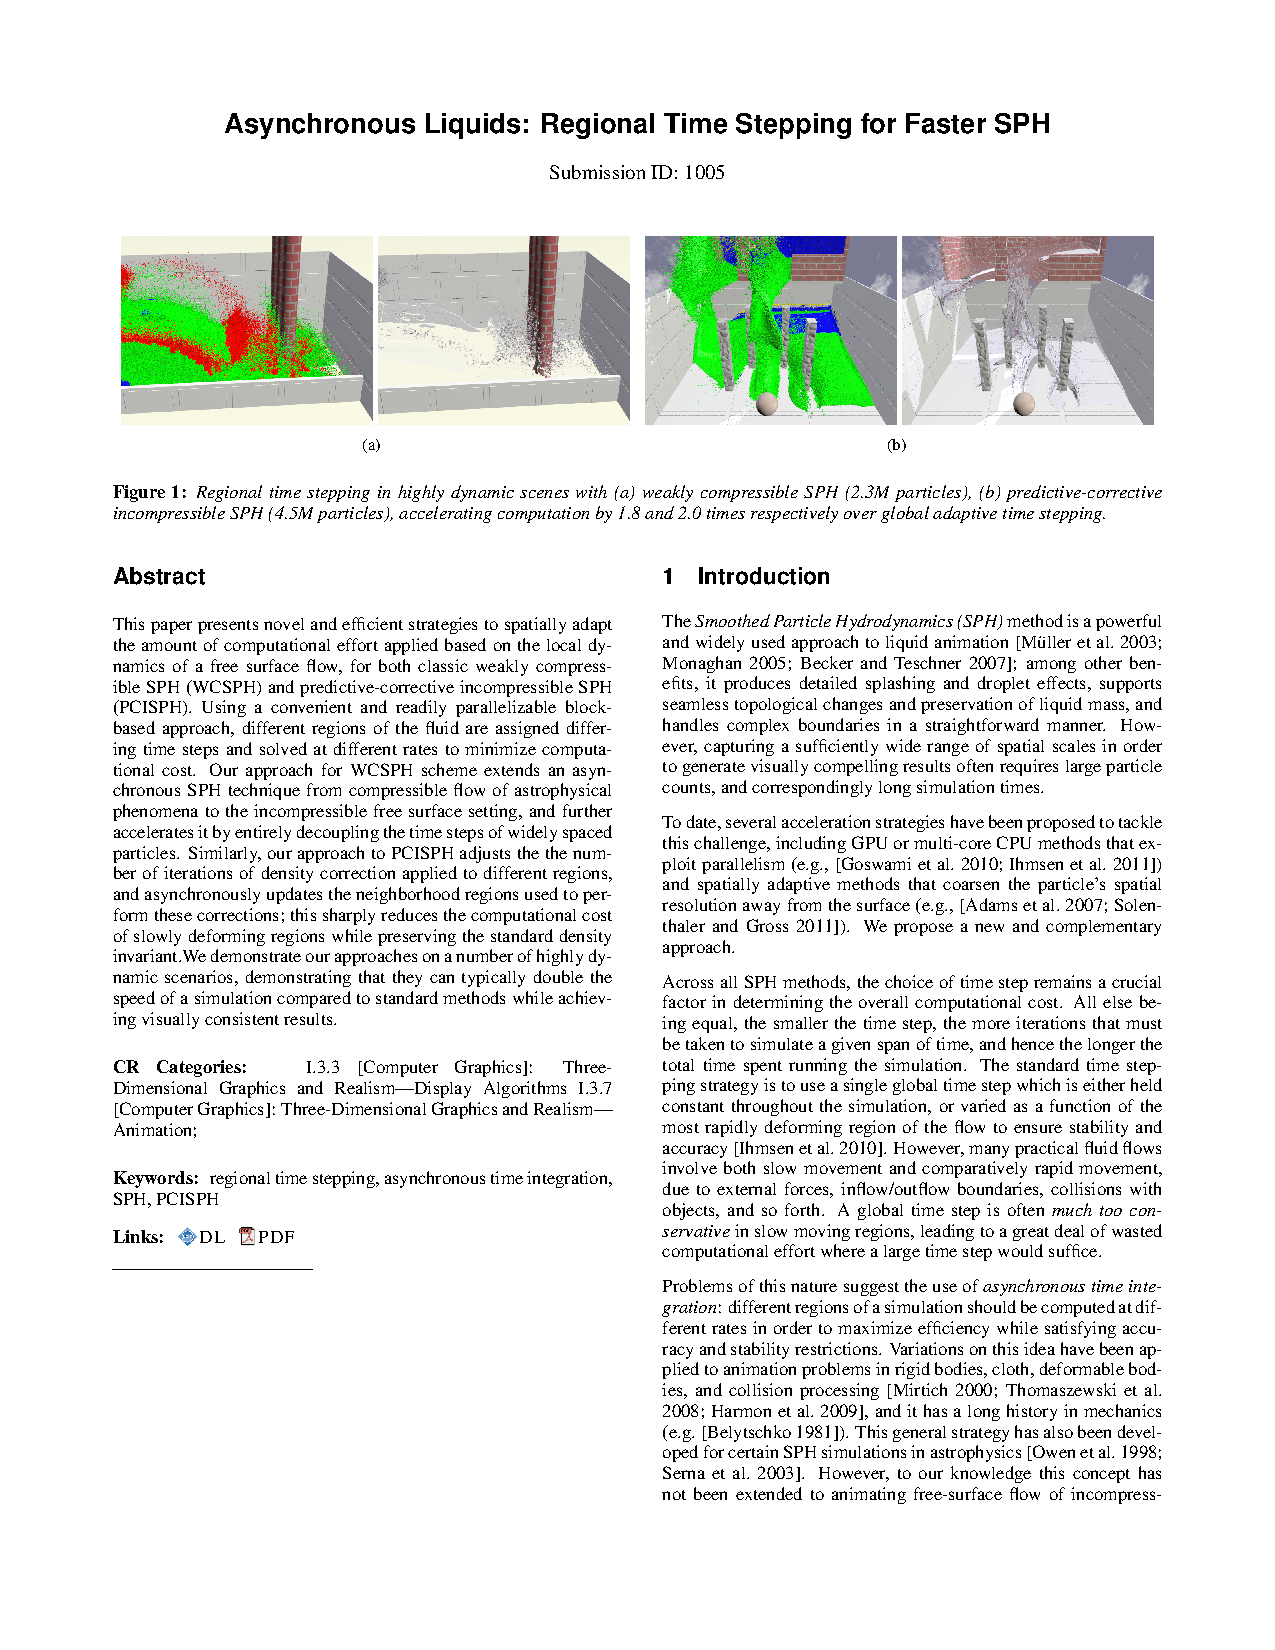
\includepdf[pages={-}]{appendices/rts.pdf}
\end{appendices}

\end{document}
